\documentclass[border=10pt]{standalone}
\usepackage[svgnames]{xcolor}
\usepackage{amsmath}
\usepackage{pgfplots}
\pgfplotsset{compat=newest}
\usepackage[sfdefault]{FiraSans}
\usepackage{FiraMono}
\renewcommand*\familydefault{\sfdefault}
\begin{document}
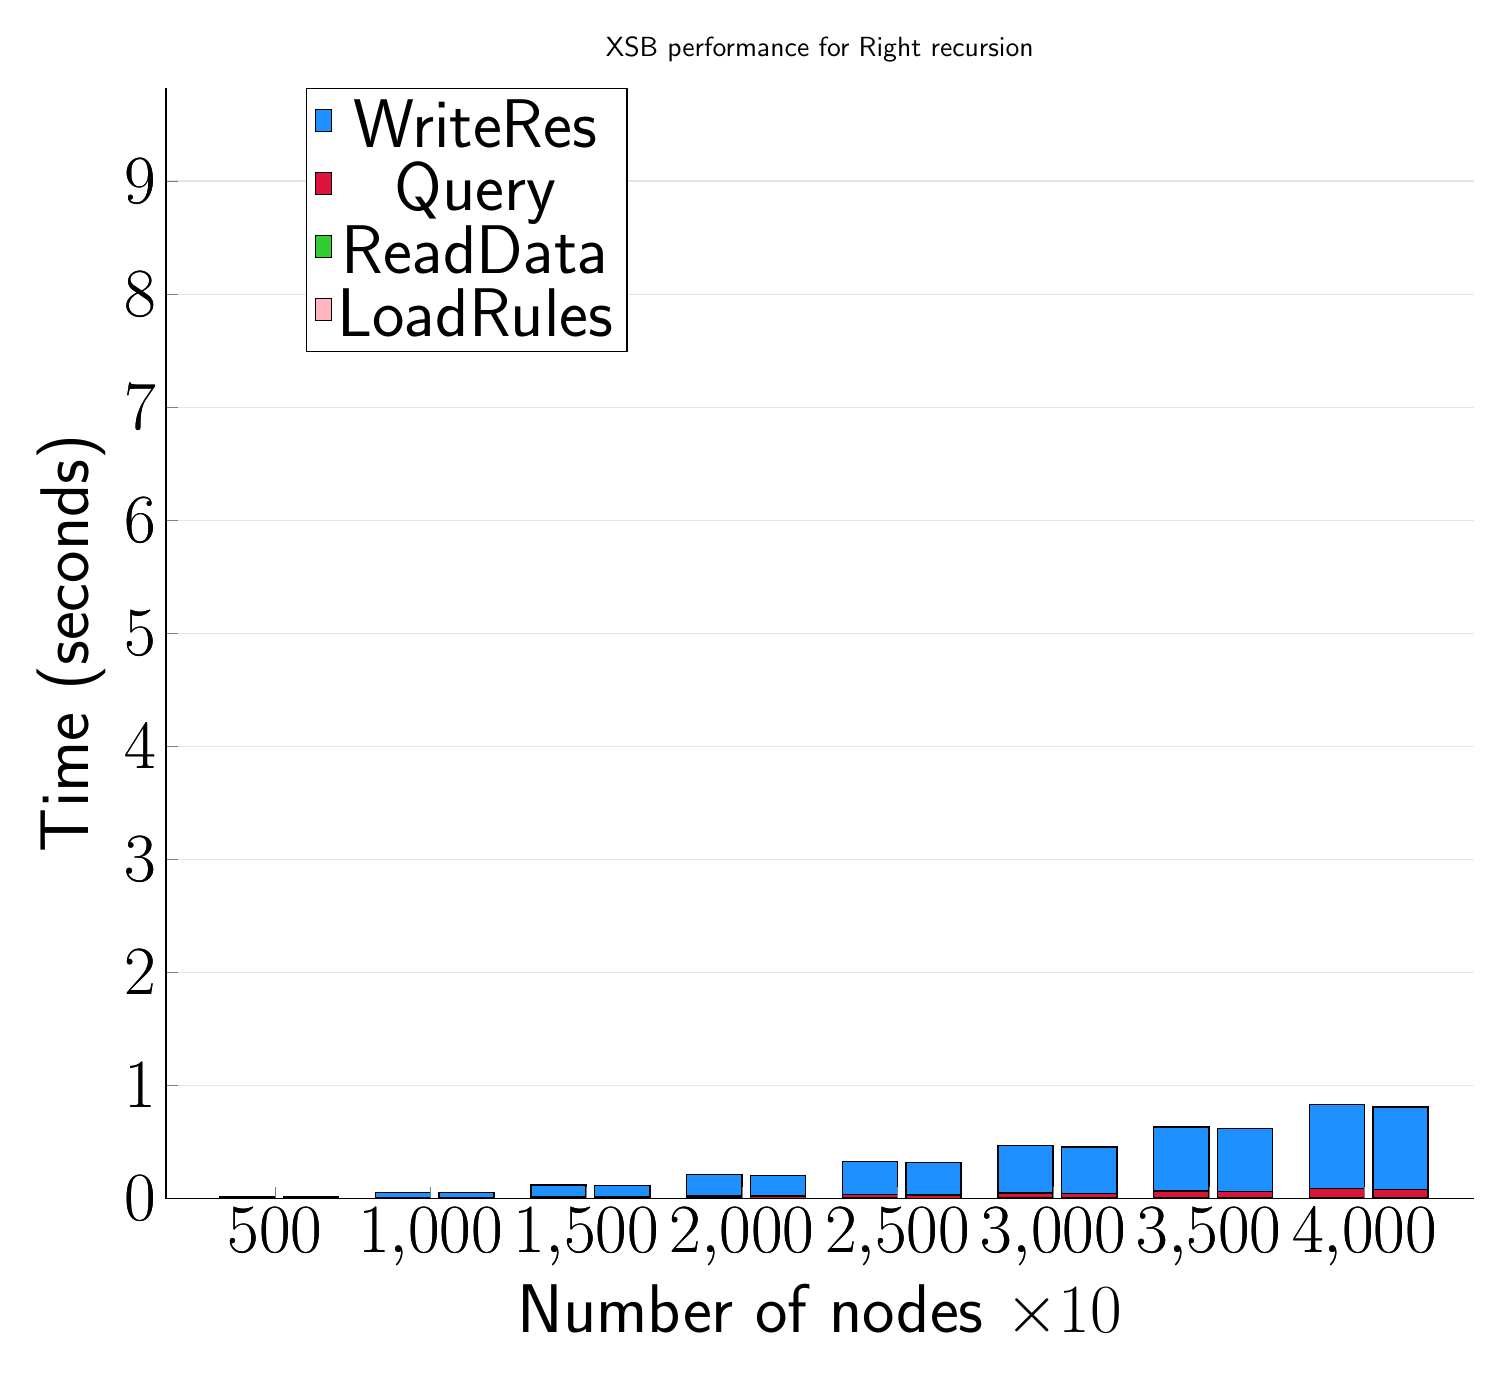
\begin{tikzpicture}
	\begin{axis}[
			ybar stacked,
			title={XSB performance for Right recursion},
			bar shift=-10pt,
			width=1.5\textwidth,
			bar width=0.7cm,
			ymajorgrids, tick align=inside,
			major grid style={draw=gray!20},
			xtick=data,
			ymin=0, ymax=9.824258804321289,
			axis x line*=bottom,
			axis y line*=left,
			enlarge x limits=0.1,
			legend style={
					at={(0.23, 1)},
					anchor=north,
					legend columns=1,
					font=\Huge,
				},
			ylabel={Time (seconds)},
			xlabel={Number of nodes $\times 10$},
			label style={font=\Huge},
			tick label style={font=\Huge},
		]
		\addlegendimage{fill=DodgerBlue, draw=black, line width=0.2pt}
		\addlegendentry{WriteRes}
		\addlegendimage{fill=Crimson, draw=black, line width=0.2pt}
		\addlegendentry{Query}
		\addlegendimage{fill=LimeGreen, draw=black, line width=0.2pt}
		\addlegendentry{ReadData}
		\addlegendimage{fill=LightPink, draw=black, line width=0.2pt}
		\addlegendentry{LoadRules}
		\addplot +[fill=LightPink, draw=black, line width=0.5pt] coordinates {
				(500, 0.0011824369430542)
				(1000, 0.001032829284667968)
				(1500, 0.0010430335998535159)
				(2000, 0.001077628135681153)
				(2500, 0.001082897186279298)
				(3000, 0.0010778665542602551)
				(3500, 0.001108765602111818)
				(4000, 0.001110315322875977)
			};
		\addplot +[fill=LimeGreen, draw=black, line width=0.5pt] coordinates {
				(500, 0.0008392810821533202)
				(1000, 0.001302146911621094)
				(1500, 0.001829743385314941)
				(2000, 0.0023759126663207997)
				(2500, 0.002809476852416992)
				(3000, 0.003381705284118652)
				(3500, 0.0038076162338256843)
				(4000, 0.004334592819213867)
			};
		\addplot +[fill=Crimson, draw=black, line width=0.5pt] coordinates {
				(500, 0.001453185081481932)
				(1000, 0.0052290201187133786)
				(1500, 0.01127848625183104)
				(2000, 0.02014231681823729)
				(2500, 0.03143727779388428)
				(3000, 0.04500451087951661)
				(3500, 0.061600399017333995)
				(4000, 0.0811652421951294)
			};
		\addplot +[fill=DodgerBlue, draw=black, line width=0.5pt] coordinates {
				(500, 0.01195979118347167)
				(1000, 0.04693729877471924)
				(1500, 0.10430402755737307)
				(2000, 0.18714234828948992)
				(2500, 0.29157564640045164)
				(3000, 0.4193634033203127)
				(3500, 0.5661097049713133)
				(4000, 0.7435030460357664)
			};
	\end{axis}
	\begin{axis}[
			ybar stacked,
			bar shift=13pt,
			width=1.5\textwidth,
			bar width=0.7cm,
			ymajorgrids, tick align=inside,
			major grid style={draw=none},
			xtick=data,
			ymin=0, ymax=9.824258804321289,
			axis x line*=none,
			axis y line*=none,
			enlarge x limits=0.1,
			label style={font=\Huge},
			tick label style={font=\Huge},
		]
		\addplot +[fill=LightPink, draw=black, line width=0.5pt] coordinates {
				(500, 0.0006356)
				(1000, 0.0005981000000000001)
				(1500, 0.0006062000000000002)
				(2000, 0.0006049000000000002)
				(2500, 0.0006134000000000002)
				(3000, 0.0006179999999999997)
				(3500, 0.0006344)
				(4000, 0.0006305)
			};
		\addplot +[fill=LimeGreen, draw=black, line width=0.5pt] coordinates {
				(500, 0.0005735000000000001)
				(1000, 0.000998)
				(1500, 0.0014479)
				(2000, 0.0019379)
				(2500, 0.0023728000000000004)
				(3000, 0.0028685000000000004)
				(3500, 0.0033207000000000006)
				(4000, 0.0037741999999999997)
			};
		\addplot +[fill=Crimson, draw=black, line width=0.5pt] coordinates {
				(500, 0.0013297)
				(1000, 0.0048419)
				(1500, 0.010437400000000001)
				(2000, 0.0185825)
				(2500, 0.028757999999999995)
				(3000, 0.0412498)
				(3500, 0.05628029999999999)
				(4000, 0.07377140000000001)
			};
		\addplot +[fill=DodgerBlue, draw=black, line width=0.5pt] coordinates {
				(500, 0.011455700000000003)
				(1000, 0.045626)
				(1500, 0.10221069999999999)
				(2000, 0.18175310000000003)
				(2500, 0.28576339999999995)
				(3000, 0.4114217)
				(3500, 0.5573236)
				(4000, 0.7303435)
			};
	\end{axis}
\end{tikzpicture}

\end{document}
